\chapter{The Standard Model}

The standard model described the interaction of quarks, leptons and gauge bosons.
The gauge boson intermediate electromagnetic, weak, and strong interaction.
In the standard model, the gauge group is $\mathrm{SU(3)}\times \mathrm{SU(2)} \times \mathrm{U(1)}$, where $\mathrm{SU(3)}$ concerns the color degrees of freedom, the $\mathrm{SU(2)}\times \mathrm{U(1)}$ is gauge group of the electroweak interaction.

The matters in the standard model consists of quarks and leptons, each of them have three generations:
\begin{equation}
	\begin{tabular}{c |c c |c c}
		\hline \hline 
		Generation & \multicolumn{2}{c|}{Quarks} & \multicolumn{2}{c}{Leptons} \\ \hline
		I & $u$ & $d$ & $e$ & $\nu_e$ \\ 
		II & $c$ & $s$ & $\mu$ & $\nu_\mu$ \\  
		III & $t$ & $b$ & $\tau$ & $\nu_\tau$ \\
		\hline \hline
	\end{tabular}
\end{equation}
The gauge theory is written as a nonabelian gauge theory, or the Yang-Mills theory, which forbid the gauge field to have mass term.
Also, the weak interaction breaks the parity -- it only involve the left-handed spinor field, and such single-handed gauge symmetry forbid the mass term for fermions.
In order to obtain the mass, the Higgs field should be introduced, which involves the spontaneous symmetry breaking.




\section{Nonabelian Gauge Theory}
The U(1)-gauge-invariant QED Lagrangian consists of the gauge part and the matter part:
\begin{equation}
\begin{aligned}
	\mathcal L_{\mathrm{QED}} &= \mathcal L_\gamma + \mathcal L_\psi \\
	&= -\frac{1}{4} F^{\mu\nu} F_{\mu\nu} + \bar\psi(i\cancel D-m)\psi.
\end{aligned}
\end{equation}
where the gauge-covariant derivative 
\begin{equation}
	D_\mu = \partial_\mu - iq A_\mu
\end{equation}
and the field strength tensor
\begin{equation}
	F_{\mu\nu} = \frac{i}{q} [D_\mu, D_\nu] = \partial_\mu A_\nu -\partial_\nu A_\mu
\end{equation}
are all manifestly invariant under U(1) gauge transformation.

The nonabelian gauge theory generalize the gauge group to be a general (nonabelian) Lie group parametrized as
\begin{equation}
	U(x) = \exp\left[-i g \pi^a(x) T^a\right],
\end{equation}
where $\{T^a\}$ are the generators of the gauge group.
For the nonabelian Lie group, the commutation relation, the Lie algebra, specify the structure of the infinitesimal gauge transformation.

\subsection{Yang-Mills Theory}
The gauge-invariant Lagrangian can be:
\begin{equation}
\begin{aligned}
	\mathcal L_{\mathrm{n.a.}} &= \mathcal L_{\mathrm{YM}} + \mathcal L_{\mathrm{matter}} \\
	&= -\frac{1}{4} F^{a,\mu\nu} F^a_{\mu\nu} + \bar\psi(i\cancel D-m)\psi.
\end{aligned}
\end{equation}
The form of Yang-Mills Lagrangian similar to the Maxwell field:
\begin{equation}
	\mathcal L_{\mathrm{YM}} = -\frac{1}{4} F^{a,\mu\nu} F^a_{\mu\nu}.
\end{equation}
To get gauge-invariant Lagrangian for the matter fields, we simply replace the ordinary derivative with the gauge-covariant derivative:
\begin{equation}
	\mathcal L_{\mathrm{matter}} = \begin{cases}
		\psi(i\gamma^\mu D_\mu - m)\psi & \text{Fermion} \\
		(D^\mu \phi)^\dagger D_\mu \phi - m^2 \phi^\dagger \phi & \text{Scalar}
	\end{cases}.
\end{equation}
The covariant derivative $D_\mu$ is now defined as
\begin{equation}
	D_\mu = \partial_\mu - i g A_\mu^a T^a,
\end{equation}
and the field-strength tensor is then
\begin{equation}
\begin{aligned}
	F^a_{\mu\nu} &= \frac{i}{g}[D_\mu, D_\nu]^a \\
	&= \partial_\mu A_\nu^a - \partial_\nu A_\nu^a -ig f^{abc} A^b_\mu A^c_\nu,
\end{aligned}
\end{equation}
The field strength tensor $F_{\mu\nu}$ transform as
\begin{equation}
	F_{\mu\nu}(x) \rightarrow U(x) F_{\mu\nu}(x) U^\dagger(x).
\end{equation}
The Lagrangian 
\begin{equation*}
	\mathcal L_{\mathrm{GI}} = -\frac{1}{2} \mathrm{Tr}\left[F_{\mu\nu} F^{\mu\nu}\right]
\end{equation*}
is manifestly gauge-invariant.
Also, we can also choose the renormalization of the generators so that $\mathrm{Tr}[T^aT^b] = \delta^{ab}$.
In this way, when express the field strength as $F_{\mu\nu} = F_{\mu\nu}^a T^a$, the above gauge-invariant Lagrangian is exactly the Yang-Mills Lagrangian $\mathcal L_{\mathrm{YM}}$.

The covariant derivative transforms as
\begin{equation}
	D_\mu \rightarrow U(x) D_\mu U^\dagger(x)
	=\partial_\mu - i g \left[U(x) A_\mu(x) U^\dagger(x) + \frac{i}{g} U(x)\partial_\mu U^\dagger(x)\right].
\end{equation}
The matter part $\mathcal L_{\mathrm{matter}}$ is invariant if we define the transformation of the gauge field as:
\begin{equation}\label{eq:SM-YM-GT-1}
	A_\mu(x) \rightarrow U(x) A_\mu(x) U^\dagger(x) + \frac{i}{g} U(x)\partial_\mu U^\dagger(x).
\end{equation}

Similar to QED case, the gauge redundancy causes trouble in quantization.
We follow the Faddeev-Popov procedure to quantize the Yang-Mills Lagrangian.

The partition function of the Yang-Mills Lagriangian is
\begin{equation}
	Z = \int D[A] \exp\left(i \int d^4x \mathcal{L}[A]\right)
	= \int D[A_{f}]\ \mathcal V_G[A] \exp\left(i \int d^4x \mathcal{L}_{\mathrm{YM}}[A_f]\right)
\end{equation}
where $A_f$ is the gauge-fixed field, and $\mathcal V_G[A]$ denotes the phase volume of the gauge redundancy.
The task is to determine $\mathcal V_G[A]$. 
This can be done by introducing a gauge-fixing condition:
\begin{equation}
	Z = \int D[\pi] \mathcal V_G[A]\int D[A] \delta(G[A^\pi]) \exp\left(i \int d^4x \mathcal{L}_{\mathrm{YM}}[A^\pi]\right),
\end{equation}
where the gauge-fixing function is 
\begin{equation}\label{eq:SM-YM-GF-1}
	G[A] = \partial^\mu A_\mu - X.
\end{equation}
Here $D[\pi]$ is the Haar measure over the Lie group.
$A^\pi$ denotes the gauge transformed field. 
Since the Lagrangian is gauge-invariant, we can simply drop a superscript, and the integral over $\pi$ field is just a number depending on $A$:
\begin{equation}
	\int D[\pi] \delta(G[A]) = \det\left(\frac{\delta G[A^\pi]}{\delta \pi}\right)^{-1}
\end{equation}
The infinitesimal version of the gauge transformation (\ref{eq:SM-YM-GT-1}) is
\begin{equation}
	A_\mu^a \rightarrow A_\mu^a +\frac{1}{g}\partial_\mu \pi^a + f^{abc}A^b_\mu \pi^b
	\equiv A_\mu + \frac{1}{g} D_\mu \pi^a,
\end{equation}
where the covariant derivative on the operator involves the adjoint representation:
\begin{equation}
	D_\mu \pi^a = \partial_\mu \pi^a + g f^{abc} A_\mu^b \pi^c = \partial_\mu -i g A_\mu^a \left(T^a_{\mathrm{adj}}\right)_{bc} \pi^c.
\end{equation}
The integral is then formally the operator determinant, and we thus know
\begin{equation}
	 \mathcal V_G[A] = \det(\partial^\mu D_\mu).
\end{equation}
This functional determinant can be regarded as the functional integral on a ``ghost'' field:
\begin{equation}
	\det(\partial^\mu D_\mu) = \int D[\bar c,c] \exp\left[i \int d^4 x\ \bar c (-\partial^\mu D_\mu)c \right].
\end{equation}
The gauge-fixing condition (\ref{eq:SM-YM-GF-1}) impose a hard constraint on the field configuration.
For our convenience, we 
\begin{equation}
\begin{aligned}
	Z &= \int DX e^{-\frac{X}{2 \xi}}\int D[A_X] \exp\left\{i\int d^4x \left[\mathcal{L}_{\mathrm{YM}} - \bar c\partial^\mu D_\mu c \right]\right\} \\
	&= \int D[A] e^{-\frac{i}{2\xi}(\partial^\mu A_\mu)^2} \exp\left\{i\int d^4x \left[\mathcal{L}_{\mathrm{YM}} -\frac{1}{2\xi}(\partial^\mu A_\mu)^2 - \bar c\partial^\mu D_\mu c \right]\right\}.
\end{aligned}
\end{equation}
The gauge-fixing results in a modified Lagrangian with gauge-fixing term and ghost term:
\begin{equation}
\begin{aligned}
	\mathcal L &= \mathcal{L}_{\mathrm{YM}} + \mathcal{L}_{\mathrm{gf}} + \mathcal{L}_{\mathrm{gh}}, \\
	\mathcal{L}_{\mathrm{gf}} &= -\frac{1}{2\xi}(\partial^\mu A_\mu)^2, \\
	\mathcal{L}_{\mathrm{gh}} &= -\bar c\partial^\mu D_\mu c.
\end{aligned}
\end{equation}

In the standard model, the weak and strong interaction is described by the SU(2) and SU(3) Yang-Mills theory respectively, so we mainly focus on the those two cases.


\subsection{SU(3) Lie Algebra}
For the fundamental representation, the generators for the SU(3) is one-half of the \textit{Gell-Mann matrices} $T^a = \frac{1}{2}\lambda^a$, $a=1,\dots,8$, where the 8 matrices are:
\begin{equation}
\begin{aligned}
	\lambda^1 &= \left[\begin{array}{ccc}
		0 & 1 & 0 \\ 1 & 0 & 0 \\ 0 & 0 & 0
	\end{array} \right], &
	\lambda^2 &= \left[\begin{array}{ccc}
		0 & -i & 0 \\ i & 0 & 0 \\ 0 & 0 & 0
	\end{array} \right], \\
	\lambda^3 &= \left[\begin{array}{ccc}
		1 & 0 & 0 \\ 0 & -1 & 0 \\ 0 & 0 & 0
	\end{array} \right], &
	\lambda^4 &= \left[\begin{array}{ccc}
		0 & 0 & 1 \\ 0 & 0 & 0 \\ 1 & 0 & 0
	\end{array} \right], \\
	\lambda^5 &= \left[\begin{array}{ccc}
		0 & 0 & -i \\ 0 & 0 & 0 \\ i & 0 & 0
	\end{array} \right], &
	\lambda^6 &= \left[\begin{array}{ccc}
		0 & 0 & 0 \\ 0 & 0 & 1 \\ 0 & 1 & 0
	\end{array} \right], \\
	\lambda^7 &= \left[\begin{array}{ccc}
		0 & 0 & 0 \\ 0 & 0 & -i \\ 0 & i & 0
	\end{array} \right], &
	\lambda^8 &= \frac{1}{\sqrt{3}}\left[\begin{array}{ccc}
		1 & 0 & 0 \\ 0 & 1 & 0 \\ 0 & 0 & -2
	\end{array} \right].
\end{aligned}
\end{equation}
The commutation relation among the generator defines the \textit{structure constant}:
\begin{equation}
	\left[T^a, T^b\right] = i f^{abc} T^c.
\end{equation}
The product of two SU(3) generators is
\begin{equation}
	T^a T^b = \frac{1}{6}\delta^{ab} + \frac{1}{2} d^{abc} T^c + \frac{i}{2} f^{abc} T^c,
\end{equation}
where
\begin{equation}
	\frac{i}{2} f^{abc} = \mathrm{Tr}\left([T^a,T^b]T^c \right), \quad
	\frac{1}{2} d^{abc} = \mathrm{Tr}\left(\{T^a,T^b\}T^c \right).
\end{equation}
The cycling properties of the trace expression leads to 
\begin{equation}
	f^{abc} = f^{bca} = f^{cab}, \quad
	d^{abc} = d^{bca} = d^{cab}.
\end{equation}
It also manifest that $f^{abc}$ is totally anti-symmetric and $d^{abc}$ totally symmetric.
This also leads to the trace identities:
\begin{equation}
\begin{aligned}
	\mathrm{Tr}(T^a T^b) &= \frac{1}{2}\delta^{ab}, \\
	\mathrm{Tr}(T^a T^b T^c) &= \frac{1}{4}(d^{abc} + if^{abc}), \\
	\mathrm{Tr}(T^a T^b T^c T^d) &= \frac{1}{12} \delta^{ab}\delta^{cd} + \frac{1}{8}(d^{abe}+if^{abe})(d^{cde}+if^{cde}).
\end{aligned}
\end{equation}

The generator in representation labeled by $R$ is denoted as $T_R^a$.
One important representation apart from the fundamental representation is the adjoint representation, which is a 8-dimensional representation defined as
\begin{equation}
	(T^a_{\mathrm{adj}})^{bc} = -i f^{abc}.
\end{equation}

Also, different representations can be characterized by the quadratic Casimir $C_2(R)$ defined as
\begin{equation}
	T^a_R T^a_R = C_2(R) \mathbbm 1.
\end{equation}
We know
\begin{equation}
	C_2(\text{fund}) = \frac{4}{3},\quad
	C_2(\text{adj}) =3.
\end{equation}
This also means
\begin{equation}
	f^{acd} f^{bcd} = 3 \delta^{ab}.
\end{equation}





\subsubsection{Roots and Weights}
For a simple Lie algebra, a standard set of generators (called the \textit{Cartan-Weyl basis}) can be chosen so that it contains a maximal number of mutually commuting subset.
The maximum number of such generators is defined as the \textit{rank} of the algebra.
The SU(3) Lie algebra is rank-2, with the Cartan-Weyl basis
\begin{equation}
	H_1 = \frac{1}{2}\lambda_3, \quad H_2 = \frac{1}{2}\lambda_8
\end{equation}
The common eigenstates of Cartan sub-algebra is denoted as $\{|\bm m\rangle\}$, where each $\bm m$ is a vector, called the \textit{weight}, defined by
\begin{equation}
	H_i |\bm m\rangle = m_i |\bm m\rangle.
\end{equation}
Apart from the Cartan sub-algebra, other generators can be linearly combined to form a standard non-Hermitian basis $\{E^\pm_{\bm \alpha}\}$.
Each element is labeled by an $r$-dimensional vectors $\pm \bm\alpha$, called the \textit{root}, which is defined by the commutation relation:
\begin{equation}
	[H_i, E_{\bm \alpha}^\pm] = \pm \alpha_i E^\pm_{\bm \alpha}.
\end{equation}
We can also denote $E_{\pm\bm{\alpha}} \equiv E_{\bm{\alpha}}^\pm$ for notational simplicity.
Note that the action of $E_\alpha$ will change the weight,
\begin{equation}
\begin{aligned}
	H_i E_{\bm \alpha}|\bm m\rangle 
	&= [H_i, E_{\bm \alpha}]|\bm m\rangle + E_{\bm \alpha} H_i |\bm m\rangle \\
	&= (m_i + \alpha_i) E_{\bm \alpha}|\bm m\rangle,
\end{aligned}
\end{equation}

For SU(3), since $\{H_i\}$ are all diagonal, the common eigenstates are
\begin{equation}
	\begin{bmatrix}
		1 \\ 0 \\ 0
	\end{bmatrix} = \left|\left(\frac{1}{2}, \frac{\sqrt{3}}{6}\right)\right\rangle, \quad
	\begin{bmatrix}
		0 \\ 1 \\ 0
	\end{bmatrix} = \left|\left(-\frac{1}{2}, \frac{\sqrt{3}}{6}\right)\right\rangle, \quad
	\begin{bmatrix}
		0 \\ 0 \\ 1
	\end{bmatrix} = \left|\left(0, -\frac{\sqrt{3}}{3}\right)\right\rangle.
\end{equation}
These vectors, plotted in a plane, form a equilateral triangle:
\begin{equation}
	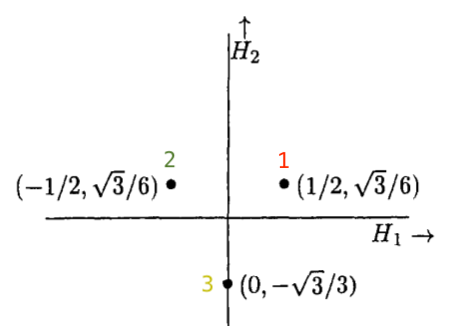
\includegraphics[width=0.35\linewidth,align=c]{pics/SM-LA-SU3-1.png}
\end{equation}
Other generators are labeled by 
\begin{equation}
	E_{\bm{\alpha}_1} = \left[\begin{array}{ccc}
		0 & 1 & 0 \\ 0 & 0 & 0 \\ 0 & 0 & 0
	\end{array}\right], \quad
	E_{\bm{\alpha}_2} = \left[\begin{array}{ccc}
		0 & 0 & 0 \\ 0 & 0 & 1 \\ 0 & 0 & 0
	\end{array}\right], \quad
	E_{\bm{\alpha}_3} = \left[\begin{array}{ccc}
		0 & 0 & 1 \\ 0 & 0 & 0 \\ 0 & 0 & 0
	\end{array}\right],
\end{equation}
where the root vectors are
\begin{equation}
	\bm{\alpha}_1 = (1, 0), \quad  
	\bm{\alpha}_2 = \left(-\frac{1}{2}, \frac{\sqrt 3}{2} \right), \quad
	\bm{\alpha}_3 = \left(\frac{1}{2}, \frac{\sqrt 3}{2} \right).
\end{equation}
The root vectors plotted in a plane form a regular hexagon:
\begin{equation}
	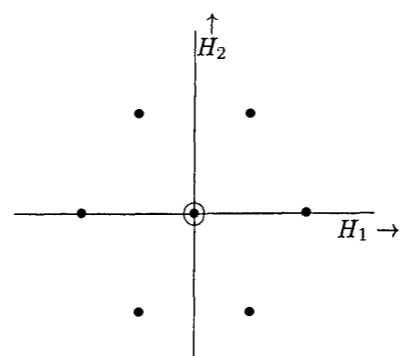
\includegraphics[width=0.35\linewidth,align=c]{pics/SM-LA-SU3-2.png}
\end{equation}

The roots of $\mathfrak{su}(3)$ are not linearly independent.
We can find a set of linear independent roots called the \textit{simple roots}.
All other roots can be expressed as a linear combination of simples roots with all positive/negative coefficients. 
The SU(3) algebra, for example, has $\bm{\alpha}_1$ and $\bm{\alpha}_2$ as its simple roots.



\subsubsection{Irreducible Representations}

An irreducible representation (Irrep) of a Lie algebra is entirely specified by the \textit{highest weight} state $|\bm M\rangle$ in the Irrep, which satisfies
\begin{equation}
	E_{\bm \alpha}|\bm M\rangle = 0
\end{equation}
for all simple root.
The Irrep then can be constructing by applying the lowering operators to the highest weight state:
\begin{equation}
	\text{Irrep} = \mathrm{span}\left\{ E_{\bm \alpha}^- E_{\bm \beta}^- \cdots E_{\bm \gamma}^- |\bm M\rangle, \ \text{all possible sequence}\right\}.
\end{equation}

The highest weight state can be systematically constructed using the tensor method.
For SU(3), we first need to introduce the complex of the fundamental representation $\bar 3$, defined by
\begin{equation}
	\exp(-i \pi^a T_{\bar 3}^a) = \exp(-i \pi^a T_{3}^a)^*,
\end{equation}
which gives
\begin{equation}
	T_{\bar 3}^a = - (T_{3}^{a})^T.
\end{equation}
The definition flip the sign of $\{H_i\}$, the weight plotted in the plane becomes the upside-down triangle:
\begin{equation}
	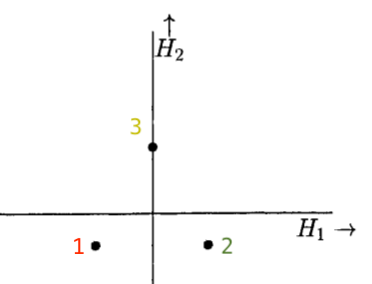
\includegraphics[width=0.35\linewidth,align=c]{pics/SM-LA-SU3-3.png}
\end{equation}
The highest wight state in $\bar 3$ is $|3\rangle$.
For a general Irrep (which can be labeled by ($m,n$)-representation), the highest weight states is
\begin{equation}
	|\bm M\rangle = \bigotimes_{i=1}^m |1\rangle_i \bigotimes_{j=m+1}^{m+n} |3\rangle_j.
\end{equation}
The ladder operators are now
\begin{equation}
	E_{\bm \alpha} = \sum_{i=1}^m E_{\bm \alpha}^{(i)} - \sum_{j=m+1}^{m+n} E^{(j)}_{-\bm \alpha}.
\end{equation}
The adjoint representation of the SU(3) is the $(1,1)$-representation. 



\subsection{Quantum Chromodynamics}
The SU(3) Yang-Mills theory describe the strong interaction, also known as the quantum chromodynamics (QCD).
The Feynman rule in QCD is very complicated.
Here we just consider the simplest tree-level process $u \bar d \rightarrow u \bar d$, corresponding to the diagram
\begin{equation}
	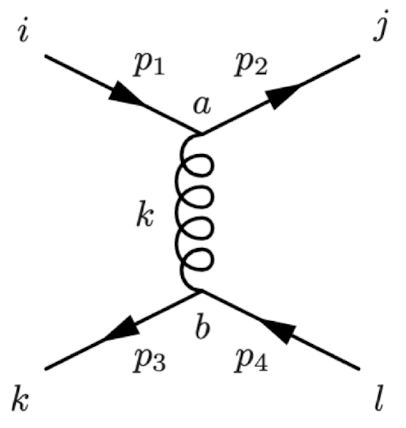
\includegraphics[width=0.2\linewidth,align=c]{pics/SM-YM-1}
	= T^a_{ji} T^a_{kl} \times (\text{QED-like term}),
\end{equation}
where the index $i$ labels the color:
\begin{equation}
	\begin{tabular}{c c c}
		\hline
		Index & Color & Simbol \\ \hline
		1 & red & $r$ \\ 
		2 & green & $g$ \\  
		3 & yellow & $y$ \\
		\hline
	\end{tabular}
\end{equation}
Since the total color is conserved in the scattering process, we can divide the color degrees of freedom to the singlet and octet, corresponding to
\begin{equation}
	3\otimes \bar 3 = 1 \otimes 8.
\end{equation}
The singlet states is
\begin{equation}
	|s\rangle = \frac{1}{\sqrt 3} \left(|r\bar r\rangle + |g\bar g\rangle + |y\bar y\rangle\right)
\end{equation}
The factor then becomes
\begin{equation}
	\left(\frac{1}{\sqrt{3}} \right)^2 (T^aT^a)_{jl} = \frac{4}{9} \delta_{jl}.
\end{equation}
For the octet state $|r \bar y\rangle$
\begin{equation}
	T^a_{i1} T^a_{3l} = -\frac{1}{6} \delta_{i1}\delta_{l3}.
\end{equation}
In QED, we know that two particle with opposite charge are attractive to each other.
From the factors above, we know that color singlet channel is attractive while the color octet channel is repulsive.
Indeed, in QCD there is phenomenon named \textit{color confinement}, which means quarks tend to form composite colorless bound state.





\subsection{Gauge Group of the Standard Model}

The standard model has $\mathrm{SU(3)}\times\mathrm{SU(2)}\times\mathrm{U(1)}$ gauge symmetry.
For a general field $\phi_{iI}$, where $i$ labels the electroweak degrees of freedom and $I$ labels the color degrees of freedom.
The covariant derivative for $\phi_{iI}$ is then
\begin{equation}
	D_\mu = \partial_\mu -i \left(g_1 B_\mu Y + g_2 W^a_\mu T^a_{2} + g_3 A_\mu^b T^b_3                                                  \right),
\end{equation}
where the operator $Y$, $T_2^a$ and $T_3^b$ is depend on the representation of U(1), SU(2) and SU(3) groups respectively. 

The weak interaction only involve left-handed spinor, so the largest fermion sector is
\begin{equation}
	Q_I = \left[
		\begin{pmatrix} u_L \\ d_L \end{pmatrix} 
		\begin{pmatrix} c_L \\ s_L \end{pmatrix} 
		\begin{pmatrix} t_L \\ b_L \end{pmatrix}
	\right]_I.
\end{equation}
Each $Q_I$ is in the $\left(3,2,\frac{1}{6}\right)$ representation, where $3$ is the fundamental representation of SU(3), $2$ is the fundamental representation of SU(2), and $\frac{1}{6}$ is the hypercharge of the U(1) gauge group.
For example the sector of first generation left-handed quarks are
\begin{equation}
	Q_1 = \begin{bmatrix}
		u_L^r & u_L^g & u_L^y \\ d_L^r & d_L^g & d_L^y
	\end{bmatrix}.
\end{equation}
Note that the electric charge satisfies
\begin{equation}
	q = I_3 + Y,
\end{equation}
where $I_3$ is the z-component of the isospin.

Besides, the left-handed leptons also involves the weak interaction but not the strong interaction
\begin{equation}
	L_I = \left[
		\begin{pmatrix} \nu_{e L} \\ e_L \end{pmatrix} 
		\begin{pmatrix} \nu_{\mu L} \\ \mu_L \end{pmatrix} 
		\begin{pmatrix} \nu_{\tau L} \\ \tau_L \end{pmatrix}
	\right]_I,
\end{equation}
and thus each $L_I$ is in the $\left(1,2,\frac{1}{2}\right)$ representation.

The right-handed quarks form $\left(3,1,\frac{2}{3}\right)$ and $\left(3,1,-\frac{1}{3}\right)$ representations, the right-handed electrons/muons/tauons form $\left(1,1,-1\right)$ representations, and the right-handed neutrinos form trivial $\left(1,1,0\right)$ representations.

In addition to the fermion, there is also a scalar Higgs field in the representation $\left(1,2,\frac{1}{2}\right)$.
Together, we say that the standard model contains the representations (only fermions in the first generation are listed):
\begin{equation}
\begin{tabular}{c|c|c}
\hline \hline
\multicolumn{2}{c|}{Particles} & Representation\tabularnewline
\hline 
\multirow{3}{*}{Quarks} & $Q_{1}$ & $(3,2,1/6)$\tabularnewline
 & $u_{R}$ & $(3,1,2/3)$\tabularnewline
 & $d_{R}$ & $(3,1,-1/3)$\tabularnewline
\hline 
\multirow{3}{*}{Leptons} & $L_{1}$ & $(1,2,-1/2)$\tabularnewline
 & $e_{R}$ & $(1,1,-1)$\tabularnewline
 & $\nu_{eR}$ & $(1,1,0)$\tabularnewline
\hline 
Higgs & $\varphi$ & $(1,2,1/2)$\tabularnewline
\hline \hline
\end{tabular}
\end{equation}




\section{Lagrangian of the Standard Model}

\subsection{Electroweak Symmetry Breaking}
Beside the quarks, leptons and gauge bosons, a doublet scalar field (Higgs) is also introduced in order to generate mass for the particles:
\begin{equation}
	\varphi \equiv \left[\begin{array}{c}
		\varphi_1 \\ \varphi_2
	\end{array} \right],
\end{equation}
which is also an isospin doublet with hyperchage $Y=\frac{1}{2}I$:
\begin{equation}
	\begin{tabular}{c c c c}
		\hline 
		Field & $I_3$ & $Y$ & $q$\\ \hline
		$\varphi_1$ & $1/2$ & $1/2$ & $1$ \\ 
		$\varphi_2$ & $-1/2$ & $1/2$ & $0$ \\  
		\hline 
	\end{tabular}
\end{equation}

The Lagrangian of the Higgs field is 
\begin{equation}\label{eq:SM-Higgs-L1}
	\mathcal L = -\frac{1}{4}(W^a_{\mu\nu})^2 - \frac{1}{4}B_{\mu\nu}^2 +(D^\mu \varphi)^\dagger D_\mu \varphi- V(\varphi),
\end{equation}
where the field strength tensors are
\begin{equation}
\begin{aligned}
	W^a_{\mu\nu} &= \partial_\mu W_\nu^1 - \partial_\nu W^1_\mu + g_2 (W_\mu^2 W_\nu^3 - W_\mu^3 W_\nu^2), \\
	W^a_{\mu\nu} &= \partial_\mu W_\nu^1 - \partial_\nu W^1_\mu + g_2 (W_\mu^3 W_\nu^1 - W_\mu^1 W_\nu^3), \\
	W^a_{\mu\nu} &= \partial_\mu W_\nu^1 - \partial_\nu W^1_\mu + g_2 (W_\mu^1 W_\nu^2 - W_\mu^2 W_\nu^1), \\
	B^a_{\mu\nu} &= \partial_\mu B_\nu^1 - \partial_\nu B^1_\mu,
\end{aligned}
\end{equation}
and the Higgs interaction is
\begin{equation}
	V(\varphi) = \frac{\lambda}{4} \left(\varphi^\dagger \varphi - \frac{v^2}{2} \right)^2.
\end{equation}
This potential gives $\varphi$ a nonzero vacuum expectation value (VEV). 
We can make a gauge transformation so that
\begin{equation}
	\varphi_0 = \langle 0| \varphi |0\rangle = \frac{v}{\sqrt 2} \left[\begin{array}{c}
		0 \\ 1	\end{array} \right].
\end{equation}


The kinetic Lagrangian is described by the SU(2) gauge-invariant Lagrangian
\begin{equation}
	\mathcal L_{\mathrm{kin}} = (D^\mu \varphi)^\dagger D_\mu \varphi,
\end{equation}
where the covariant derivative is
\begin{equation}
	D_\mu = \partial_\mu -i \left(g_1 B_\mu Y + g_2 W^a_\mu T_2^a\right).
\end{equation}
We can introducing the Weinberg angle
\begin{equation}
	\theta_W \equiv\arctan \frac{g_1}{g_2},
\end{equation}
and the fields
\begin{equation}
\begin{aligned}
	W_\mu^\pm &\equiv \frac{1}{\sqrt 2}(W^1_\mu \mp i A_\mu^2), \\
	Z_\mu &\equiv \cos{\theta_W} W^3_\mu - \sin{\theta_W} B_\mu, \\
	A_\mu &\equiv \sin{\theta_W} W_\mu^3 + \cos{\theta_W} B_\mu.
\end{aligned}
\end{equation}
The reverse transformation for $W_\mu^3$ and $B_\mu$ is
\begin{equation}
\begin{aligned}
	W_\mu^3 &= \cos{\theta_W} Z_\mu + \sin{\theta_W} A_\mu, \\
	B_\mu &= -\sin{\theta_W} Z_\mu +\cos{\theta_W} A_\mu.
\end{aligned}
\end{equation}
The off-diagonal part of the Lie algebra becomes
\begin{equation}
	\frac{1}{\sqrt 2}\begin{bmatrix}
		0 &  W^+_\mu \\
		W_\mu^- & 0
	\end{bmatrix},
\end{equation}
and the diagonal part becomes
\begin{equation}
\begin{aligned}
	g_2 W_\mu^3 T^z_2 + g_1 B_\mu Y
	&= g_2 (\cos{\theta_W} Z_\mu + \sin{\theta_W} A_\mu) T^3_2 + g_1 Y (-\sin{\theta_W} Z_\mu +\cos{\theta_W} A_\mu) \\
	&= g_2 \cos{\theta_W} A_\mu \left(T^3_2 + Y\right) + eZ_\mu \left(\cot{\theta_W}T_2^3 - \tan{\theta_W}Y \right) \\
	&= e A_\mu q + \frac{e}{\sin{\theta_W}\cos{\theta_W}} Z_\mu \left(\cos^2{\theta_W}T_2^3 - \sin^2{\theta_W} Y\right) \\
	&= e A_\mu q + \frac{e}{\sin{\theta_W}\cos{\theta_W}} Z_\mu \left(T_2^3 - \sin^2{\theta_W} q\right).
\end{aligned}
\end{equation}
Note that the gauge field $A_\mu$ describe QED, so we identify the coupling constant with the electric charge:
\begin{equation}
	e = g_2 \sin{\theta_W} = g_1 \cos{\theta_W}.
\end{equation}

For Higgs field, 
\begin{equation}
	T^3_2 = \frac{1}{2}\sigma^z, \quad
	Y = \frac{1}{2} I,\quad 
	q = \begin{bmatrix}
		1 & 0 \\ 0 & 0
	\end{bmatrix}.
\end{equation}
$T^3_2 = \frac{1}{2}\sigma^z$, $Y=\frac{1}{2}I$, so 
With the new definition of the field, the Lie algebra of becomes
\begin{equation}
\begin{aligned}
	g_2 W^a_\mu T_2^a + g_1 B_\mu Y 
	&= \frac{e}{2 \sin{\theta_W}} 
	\begin{bmatrix}
		2\sin{\theta_W} A_\mu + \frac{\cos{2\theta_W}}{\cos{\theta_W}} Z_\mu & \sqrt{2} W^+_\mu \\
		\sqrt{2} W_\mu^- & \frac{1}{\cos{\theta_W}} Z_\mu
	\end{bmatrix}.
\end{aligned}
\end{equation}
We can now expand the kinetic term to get the effective mass of the the gauge field in unitary gauge. 
The mass term is the quadratic part of $\varphi$:
\begin{equation}
\begin{aligned}
	\mathcal L_{\mathrm{mass}} 
	&= \varphi_0^\dagger \left(g_2 W^a_\mu T_2^a + g_1 B_\mu Y\right)^2 \varphi_0 \\
	&= \frac{e^2v^2}{8 \sin^2{\theta_W}} 
	\begin{bmatrix}
		0 & 1
	\end{bmatrix} 
	\begin{bmatrix}
		\cdots & \sqrt{2} W^+_\mu \\
		\sqrt{2} W_\mu^- & \frac{1}{\cos{\theta_W}} Z_\mu
	\end{bmatrix}^2
	\begin{bmatrix}
		0 \\ 1
	\end{bmatrix} \\
	&= m_W W^{+\mu} W_\mu^- + \frac{1}{2}m_Z^2 Z^\mu Z_\mu,
\end{aligned}
\end{equation}
where the mass for $W$ and $Z$ bosons are
\begin{equation}
	m_W = \frac{ev}{2 \sin{\theta_W}}, \quad 
	m_Z = \frac{e v}{2\sin{\theta_W}\cos{\theta_W}} = \frac{m_W}{\cos{\theta_W}}.
\end{equation}
Note that the photon field $A_\mu$ does not obtain mass from the Higgs field.



\subsection{Higgs-Gauge Sector}
We are now going to express the Lagrangian (\ref{eq:SM-Higgs-L1}) in terms of the fields we have just introduced.
In the unitary gauge, the Higgs field can be written as
\begin{equation}
	\varphi = \frac{1}{\sqrt 2} \begin{bmatrix}
		v + H(x) \\ 0
	\end{bmatrix},
\end{equation}
where $H(x)$ is a real scalar field.
The interaction terms gives
\begin{equation}
\begin{aligned}
	V(H) &= \frac{\lambda v^2}{4} H^2 + \frac{\lambda v}{4}H^3 + \frac{\lambda}{16}H^4 \\
	&= \frac{1}{2}m_H^2 H^2 + \frac{m_H^2}{2v} H^3 + \frac{m_H^2}{8v^2}H^4,
\end{aligned} 
\end{equation}
where we have defined the Higgs mass
\begin{equation}
	m_H^2 = \frac{\lambda v^2}{2}.
\end{equation}
Also, the fluctuation around the $\varphi_0$ also create coupling between Higgs field and the gauge fields.
We can simply replace $v^2$ with $(v+H)^2$ in the gauge field mass term to capture the coupling.
Thus, the Lagrangian is
\begin{equation}
	\mathcal L_{\mathrm{H}} = \partial^\mu H^\dagger \partial_\mu H - V(H) + \left(m_W W^{+\mu} W_\mu^- + \frac{1}{2}m_Z^2 Z^\mu Z_\mu \right) \left(H^2+2vH \right).
\end{equation}
Now consider the Lagrangian for the gauge field
\begin{equation}
	\mathcal L_{\mathrm{G}} = -\frac{1}{4}(W^a_{\mu\nu})^2 - \frac{1}{4}B_{\mu\nu}^2 + m_W W^{+\mu} W_\mu^- + \frac{1}{2}m_Z^2 Z^\mu Z_\mu.
\end{equation}
We can regroup the field strength as
\begin{equation}
\begin{aligned}
	W^+_{\mu\nu} &= D_\mu W_\nu^+ - D_\nu W^+_\mu, \\
	W^-_{\mu\nu} &= D_\mu^\dagger W_\nu^- - D_\nu^\dagger W^-_\mu, \\
	W^3_{\mu\nu} &= \sin{\theta_W} F_{\mu\nu} + \cos{\theta_W}Z_{\mu\nu} -ig_2(W^+_\mu W^-_\nu - W_\mu^- W_\nu^+), \\
	B^a_{\mu\nu} &= \cos{\theta_W} F_{\mu\nu} - \sin{\theta_W} Z_{\mu\nu},
\end{aligned}
\end{equation}
where we have defined 
\begin{equation}
\begin{aligned}
	W^\pm_{\mu\nu} &= \frac{1}{\sqrt 2} (W^1_{\mu\nu} \mp i W^2_{\mu\nu}), \\
	F_{\mu\nu} &= \partial_\mu A_\nu - \partial_\nu A_\mu, \\
	Z_{\mu\nu} &= \partial_\mu Z_\nu - \partial_\nu Z_\mu.
\end{aligned}
\end{equation}
The covariant derivative for $W^\pm$ field is
\begin{equation}
\begin{aligned}
	D_\mu &= \partial_\mu -i g_2 W^3_\mu \\
	&= \partial_\mu -i g_2 \left(\sin{\theta_W}A_\mu + \cos{\theta_W} Z_\mu \right) \\
	&= \partial_\mu -i e \left(A_\mu + \cot{\theta_W} Z_\mu \right)
\end{aligned}
\end{equation}
So the Lagrangian for the gauge field is
\begin{equation}
\begin{aligned}
	\mathcal L_\mathrm{G}
	=&\ -\frac{1}{4}(2W_{\mu\nu}^+ W^{-\mu\nu} + W_{\mu\nu}^3 W^{3\mu\nu}) -\frac{1}{4} B_{\mu\nu}B^{\mu\nu} + m_W W^{+\mu} W_\mu^- + \frac{1}{2}m_Z^2 Z^\mu Z_\mu \\
	=&\ -\frac{1}{4}(F_{\mu\nu}F^{\mu\nu} + Z_{\mu\nu} Z^{\mu\nu}) - D^{\mu} W^{+\nu} D^\dagger_\mu W_\nu^- + D^\mu W^{+\nu} D^\dagger_\nu W^-_\mu \\
	&\ +ie (F^{\mu\nu} + \cot{\theta_W} Z^{\mu\nu})W_\mu^+ W_\nu^- + m_W W^{+\mu} W_\mu^- + \frac{1}{2}m_Z^2 Z^\mu Z_\mu \\
	&\ -\frac{e^2}{2\sin^2{\theta_W}} \left(W^{+\mu}W^-_\mu W^{+\nu}W^-_\nu - W^{+\mu}W^+_\mu W^{-\nu}W^-_\nu \right).
\end{aligned}
\end{equation}
We remark that in the unitary gauge, there is no redundancy of the gauge field.
No ghost field is needed in the quantization procedure.


\subsection{Yukawa Coupling and Fermion Mass}
The fermion fields in the electroweak interaction
\begin{equation}
	\begin{tabular}{c c c c}
		\hline 
		Field & $I_3$ & $Y$ & $q$\\ \hline
		$u_L$ & $1/2$ & $1/6$ & $2/3$ \\ 
		$d_L$ & $-1/2$ & $1/6$ & $-1/3$ \\  
		$u_R$ & $0$ & $2/3$ & $2/3$ \\
		$d_R$ & $0$ & $-1/3$ & $-1/3$ \\ \hline
		$e_L$ & $-1/2$ & $-1/2$ & $-1$ \\ 
		$\nu_{eL}$ & $1/2$ & $-1/2$ & $0$ \\  
		$e_R$ & $0$ & $-1$ & $-1$ \\
		$\nu_{eR}$ & $0$ & $0$ & $0$ \\
		\hline 
	\end{tabular}
\end{equation}

The kinetic term for the fermion Lagrangian is
\begin{equation}
\begin{aligned}
	\mathcal L_{\mathrm{kin}}
	=&\ i Q^\dagger_J \sigma^\mu D_\mu Q_J + i u_{RJ}^\dagger \bar\sigma^\mu D_\mu u_{RJ} + i d_{RJ}^\dagger \bar\sigma^\mu D_\mu d_{RJ} \\
	& + i L^\dagger_J \sigma^\mu D_\mu L_J + i e_{RJ}^\dagger \bar\sigma^\mu D_\mu e_{RJ} + i \nu_{RJ}^\dagger \bar\sigma^\mu D_\mu \nu_{RJ},
\end{aligned}
\end{equation}
where we have use the index $J$ to label the generation of the fermion:
\begin{equation}
\begin{aligned}
	u_{RJ} &= \{u_R, c_R, t_R\}, & 
	d_{RJ} &= \{d_R, s_R, b_R\}, \\
	e_{RJ} &= \{e_R, \mu_R, \tau_R\}, &
	\nu_{RJ} &= \{\nu_{eR},\nu_{\mu R},\nu_{\tau R}\}.
\end{aligned}
\end{equation}

The left-handed SU(2) gauge symmetry forbid any fermion mass term, which is incompatible with the reality.
However, fermion can obtain fermion mass by introducing Yukawa coupling between the Higgs and fermion fields.

\subsubsection{Quark Sector}
The Yukawa coupling between quark and Higgs is
\begin{equation}
	\mathcal L_{q,\mathrm{Yuk}}
	= - \varepsilon^{ij} Y^u_{IJ} Q^\dagger_{iI} \varphi^\dagger_j u_{RJ}
	- Y^d_{IJ} Q^\dagger_{I} \varphi d_{RJ} +h.c..
\end{equation}
The first term corresponds to
\begin{equation}
	\left(\bar 3, \bar 2, -\frac{1}{6}\right) \times \left(1, \bar 2, -\frac{1}{2}\right) \times \left(3, 1, \frac{2}{3}\right) = \left(1,1,0\right)\oplus \cdots,
\end{equation}
with $\varepsilon^{ij}$ being the Clebsch-Gordan coefficient, and the second term corresponds to
\begin{equation}
	\left(\bar 3, \bar 2, -\frac{1}{6}\right) \times \left(1, 2, \frac{1}{2}\right) \times \left(3, 1, -\frac{1}{3}\right) = \left(1,1,0\right).
\end{equation}
Now substitute $\varphi$ with 
\begin{equation}
	\varphi = \frac{1}{\sqrt 2} \begin{bmatrix}
		0 \\ v+H
	\end{bmatrix}.
\end{equation}
The Yukawa potential then gives quark mass term:
\begin{equation}
	\mathcal L_{Q,\mathrm{Yuk}}
	= -\frac{v+H}{\sqrt 2} \left( Y^u_{IJ} u^\dagger_{LI} u_{RJ} +Y^d_{IJ} d^\dagger_{LI} d_{RJ} \right) +h.c..
\end{equation}
We can then use a basis transformation (singular value decomposition) to diagonalize the coupling matrix:
\begin{equation}
	Y^u_{IJ} = U_u M_u K^\dagger_u, \quad
	Y^d_{IJ} = U_d M_d K^\dagger_d,
\end{equation}
where $M_u$ and $M_d$ are diagonal matrices.
We can change the basis
\begin{equation}
\begin{aligned}
	u_L &\rightarrow U_u u_L, & u_R &\rightarrow K_u u_R, \\
	d_L &\rightarrow U_d d_L, & d_R &\rightarrow K_d d_R,
\end{aligned}
\end{equation}
and define the diagonal masses:
\begin{equation}
	m_{u_I} = \frac{v}{\sqrt 2} (M_u)_{II}, \quad 
	m_{d_I} = \frac{v}{\sqrt 2} (M_d)_{II},
\end{equation}
then the Lagrangian in the quark sector can be expressed as:
\begin{equation}
\begin{aligned}
	\mathcal L_Q =&\ \sum_I \bar u_I\left(i\cancel D^c-m_{u_I}\right)u_I + \sum_I \bar d_I \left(i \cancel D^c-m_{d_I}\right)d_I \\
	& -\frac{H}{v} \sum_I\left(m_{u_I}\bar u_I u_I+m_{d_I}\bar d_I d_I \right) + \mathcal L_{Q-G},
\end{aligned}
\end{equation}
where $\cancel D^c$ is the covariant derivative in QCD (neglecting the electroweak gauge), and $\mathcal L_{Q-G}$ denotes the coupling between quarks and the gauge fields.

\subsubsection{Lepton Sector}
The coupling between Higgs and $e_R$ has the general Yukawa form:
\begin{equation}
	\mathcal L_{e,\mathrm{Yuk}} = -Y^e_{IJ} L_{iI}^\dagger \varphi_j e_{R iJ} + h.c.,
\end{equation}
where $y_{IJ}$ is the Hermitian coupling matrix on generation space.
The Yukawa coupling term corresponds to
\begin{equation}
	\left(\bar 2, \frac{1}{2}\right) \times \left(2, \frac{1}{2}\right) \times \left(1, -1\right) = \left(1,0\right),
\end{equation}
which is indeed a singlet under gauge transformation (it is also a singlet under Lorentz transformation).
The Higgs field then produce the term
\begin{equation}
	\mathcal L_{e,\mathrm{Yuk}} = -\frac{Y^e_{IJ}}{\sqrt 2}(v+H) e_{LI}^\dagger e_{RJ} + h.c.,
\end{equation}
We then diagonalize the coupling matrix:
\begin{equation}
	 Y^e_{IJ} = \left[U_{e} M_e K^\dagger_{e}\right]_{IJ},
\end{equation}
where $M_e$ is diagonal.
We can then change the basis by
\begin{equation}
\begin{aligned}
	e_R &\rightarrow K_e e_R, \\
	e_L &\rightarrow U_e e_L,
\end{aligned}
\end{equation}
Then the coupling gives the mass:
\begin{equation}
	\mathcal L_{e,\mathrm{Yuk}} 
	= - \sum_I m_{e_I} \bar e_I e_I - \frac{1}{v}\sum_I m_{e_I} H \bar e_I e_I,
\end{equation}
where
\begin{equation}
	m_{e_I} = \frac{v}{\sqrt 2} (M_e)_{II}.
\end{equation}

Now we consider the neutrino mass, which is much smaller than electrons.
The neutrinos can similarly obtain mass by coupling to Higgs field.
However, as there is no gauge symmetry constraint on neutrinos, the Yukawa coupling can be
\begin{equation}
	\mathcal L_{\nu,\mathrm{Yuk}} = - Y^\nu_{IJ} \varepsilon^{ij} L_{iI} \varphi_j \nu_{RJ} - \frac{1}{2} M_{IJ} \nu_{RI} \nu_{RJ} + h.c..
\end{equation}
The first term corresponds to
\begin{equation}
	\left(2, -\frac{1}{2}\right) \times \left(2, \frac{1}{2}\right) \times \left(1, 0\right) = \left(1,0\right) \oplus(3,0),
\end{equation}
and $\varepsilon^{ij}$ is the Clebsch-Gordan coefficients.
The second term is automatically a gauge singlet.
We note here that the left-handed neutrino do not participate in any interaction, so we can neglect it in the standard model.
The only role it plays is to generate neutrino mass.

The Yukawa potential gives
\begin{equation}
	\mathcal L_{\nu,\mathrm{mass}} = -\frac{1}{2}
	\begin{bmatrix}
		\nu_L & \nu_R
	\end{bmatrix} 
	\begin{bmatrix}
		0 & Y^\nu \\ Y^{\nu\dagger} & M
	\end{bmatrix} 
	\begin{bmatrix}
		\nu_L \\ \nu_R
	\end{bmatrix}.
\end{equation}
If $M \gg m$, the eigenvalues of the mass term will be a huge masses plus some tiny masses.
In general, the low-energy part of the mass term is
\begin{equation}
	\mathcal L_{\nu,\mathrm{mass}} = -\frac{1}{2} (M_\nu)_{IJ} \left(\nu_{LI} \nu_{LJ} + \nu_{LI}^\dagger \nu_{LJ}^\dagger\right)\left(1+\frac{H}{v}\right)^2,
\end{equation}
where
\begin{equation}
	(M_\nu)_{IJ} = \frac{v^2}{2} \left(Y^{\nu T} M^{-1} Y \right)_{IJ}.
\end{equation}
We can also diagonalize the matrix $M_\nu$ by a unitary matrix $U_\nu$, corresponding to
\begin{equation}
	\nu_L \rightarrow U_\nu \nu_L.
\end{equation}

With the discussion above, we can write down the Lagrangian in the lepton sector:
\begin{equation}
\begin{aligned}
	\mathcal L_L =&\ \sum_I \bar e_I (i\cancel\partial-m_{e_I})e_I + \sum_I \left[i\nu_{LI}^\dagger \bar\sigma^\mu \partial_\mu \nu_{LI} - \frac{1}{2}m_{\nu_I} \left(\nu_L \nu_L + \nu_L^\dagger \nu_L^\dagger\right)\right] \\
	& -\frac{H}{v} \sum_I \left(m_{e_I} \bar e_I e_I + m_{\nu_I}\bar\nu_{LI}\nu_{LI}\right)+ \mathcal L_{L-G},
\end{aligned}
\end{equation}
where $\mathcal L_{L-G}$ is the lepton-gauge coupling term.



\subsection{Gauge-Current Coupling}
Using the formula
\begin{equation}
\begin{aligned}
	g_2 \sum_{a=1}^2 W^a_\mu T^a_2 &= \frac{e}{\sqrt{2}\sin{\theta_W}}\begin{bmatrix}
		0 & W_\mu^+ \\ W_\mu^- & 0
	\end{bmatrix}, \\
	g_2 W_\mu^3 T^z_2 + g_1 B_\mu Y
	&= e A_\mu q + \frac{e}{\sin{\theta_W}\cos{\theta_W}} Z_\mu \left(T_2^3 - \sin^2{\theta_W} q\right).
\end{aligned}
\end{equation}
The coupling terms $\mathcal L_{Q-G}$ and $\mathcal L_{L-G}$ are then of the form:
\begin{equation}
\begin{aligned}
	\mathcal L_{Q-G} &= \frac{e}{\sqrt{2}\sin{\theta_W}} \left(W^{+}_\mu J_Q^{-\mu} + W^{-}_\mu J_Q^{+\mu} \right) + e A_\mu J^{\mu}_{\mathrm{EM},Q} + \frac{e}{\sin{\theta_W}\cos{\theta_W}} Z_\mu J^\mu_{z,Q}, \\
	\mathcal L_{L-G} &= \frac{e}{\sqrt{2}\sin{\theta_W}}\left(W^{+}_\mu J_L^{-\mu} + W^{-}_\mu J_L^{+\mu} \right) + e A_\mu J^{\mu}_{\mathrm{EM},L} + \frac{e}{\sin{\theta_W}\cos{\theta_W}} Z_\mu J^\mu_{z,L}.
\end{aligned}
\end{equation}
Note that the off-diagonal current $J^\pm$ will change under the basis transformation $U_{IJ}$, i.e., the transformation mixes different generations:
\begin{equation}
\begin{aligned}
	J^{-\mu}_Q &= (V_Q)_{IJ} u_{LI}^\dagger \bar\sigma^\mu d_{LJ}, \\
	J^{+\mu}_Q &= (V^\dagger_Q)_{IJ} d_{LI}^\dagger \bar\sigma^\mu u_{LJ}, \\
	J^{-\mu}_L &= (V_L)_{IJ} \nu_{LI}^\dagger \bar\sigma^\mu e_{LJ}, \\
	J^{+\mu}_L &= (V^\dagger_L)_{IJ} e_{LI}^\dagger \bar\sigma^\mu \nu_{LJ},
\end{aligned}
\end{equation}
where the mixing matrices are defined as
\begin{equation}
	V_Q \equiv U^\dagger_u U_d, \quad
	V_L \equiv U_\nu^\dagger U_e.
\end{equation}

The diagonal part is invariant under the basis transformation:
\begin{equation}
\begin{aligned}
	J^\mu_{\mathrm{EM},Q} &= \frac{2}{3} u_{LI}^\dagger \bar\sigma^\mu u_{LI} - \frac{1}{3} d_{LI}^\dagger \bar\sigma^\mu d_{LI} \\
	J^\mu_{\mathrm{EM},L} &= - e_{LI}^\dagger \bar\sigma^\mu e_{LI} \\
	J_{z,Q}^\mu &= \frac{1}{2} u_{LI}^\dagger \bar\sigma^\mu u_{LI} - \frac{1}{2} d_{LI}^\dagger \bar\sigma^\mu d_{LI} J^\mu_3-\sin^2{\theta_W}J_{\mathrm{EM},Q}^\mu, \\
	J_{z,L}^\mu &= \frac{1}{2} \nu_{LI}^\dagger \bar\sigma^\mu \nu_{LI} - \frac{1}{2} e_{LI}^\dagger \bar\sigma^\mu e_{LI} J^\mu_3-\sin^2{\theta_W}J_{\mathrm{EM},L}^\mu.
\end{aligned}
\end{equation}

Finally, we can sum over the current, and write down the total fermion-gauge coupling:
\begin{equation}
	\mathcal L_{F-G} = \frac{e}{\sqrt{2}\sin{\theta_W}} \left(W^{+}_\mu J^{-\mu} + W^{-}_\mu J^{+\mu} \right) + e A_\mu J^{\mu}_{\mathrm{EM}} + \frac{e}{\sin{\theta_W}\cos{\theta_W}} Z_\mu J^\mu_{z}.
\end{equation}
From the current-gauge coupling, we can recover the effective 4-fermion theory by integrating out the gauge field.
In the low energy regime ($p^2 \ll m_W^2$), the vertex function for electron decay is:
\begin{equation}
	2\left(\frac{e}{\sqrt{2}\sin{\theta_W}} \right)^2 J^+_\mu \frac{g^{\mu\nu}}{p^2-m_W^2} J^-_\nu 
	\simeq \frac{e^2}{m_W^2 \sin^2{\theta_W}} J^{+\mu} J^-_\mu.
\end{equation}
The diagonal part of the vertex is
\begin{equation}
	\left(\frac{e}{\sin{\theta_W}\cos{\theta_W}} \right)^2 J^z_\mu \frac{g^{\mu\nu}}{p^2-m_Z^2} J^z_\nu 
	\simeq -\frac{e^2}{m_Z^2 \sin^2{\theta_W}\cos^2{\theta_W}} J^{z\mu} J^z_\mu.
\end{equation}\
Note that $m_Z^2\cos^2{\theta_W} = m_W^2$, we can then identify the fermion constant
\begin{equation}
	\frac{4G_F}{\sqrt 2} = -\frac{e^2}{m_W^2 \sin^2{\theta_W}},
\end{equation}
and the 4-Fermion vertex is
\begin{equation}
	\mathcal L_{4F} = -\frac{4G_F}{\sqrt 2} \left(J^{+\mu} J_\mu^- + J^{z\mu} J_\mu^z \right).
\end{equation}
















